\documentclass[11pt,a4paper]{article}

% Essential Packages
\usepackage[utf8]{inputenc}
\usepackage[margin=1in]{geometry}
\usepackage{amsmath,amssymb,amsfonts}
\usepackage{graphicx}
\usepackage{booktabs}
\usepackage{microtype}
\usepackage{hyperref}
\usepackage{tikz}
\usetikzlibrary{positioning}
\usepackage{listings}
\usepackage{xcolor}

% Hyperlink configuration
\hypersetup{
    colorlinks=true,
    linkcolor=blue!70!black,
    citecolor=blue!70!black,
    urlcolor=blue!70!black
}

% Code Listing Configuration
\definecolor{codegray}{rgb}{0.95,0.95,0.95}
\definecolor{codepurple}{rgb}{0.58,0,0.82}

\lstset{
    backgroundcolor=\color{codegray},
    basicstyle=\ttfamily\small,
    breaklines=true,
    keywordstyle=\color{blue},
    stringstyle=\color{codepurple},
    commentstyle=\color{green!60!black},
    frame=single,
    numbers=left,
    numberstyle=\tiny\color{gray}
}

% Document Metadata
\title{\textbf{LaTeX Development Environment on NixOS}}
\author{\textbf{NixOS \& Devenv Workspace}}
\date{\today}

\begin{document}

\maketitle

\begin{abstract}
	This document serves as a demonstration and verification of the LaTeX development environment powered by NixOS and \texttt{devenv}. It showcases mathematical typesetting, code listings, vector graphics via TikZ, and bibliographic references.
\end{abstract}

\section{Introduction}
Setting up LaTeX environments with all required packages and dependencies can be challenging across different distributions. By using NixOS and \texttt{devenv}, we achieve reproducible, hermetic development shells containing TeX Live, LSP tools (\texttt{texlab}), and build automation (\texttt{latexmk}).

As noted by Leslie Lamport~\cite{lamport1986latex}, LaTeX provides an intuitive approach to structured document layout, while NixOS~\cite{nixos2004} ensures exact package reproducibility.

\section{Mathematical Formulations}
LaTeX excels at mathematical notation. For example, Euler's identity is given by:
\begin{equation}
	e^{i\pi} + 1 = 0
\end{equation}

We can also express the Gaussian integral:
\begin{equation}
	\int_{-\infty}^{\infty} e^{-x^2} \, dx = \sqrt{\pi}
\end{equation}

\section{TikZ Diagram Example}
Below is a simple architecture diagram rendered natively using TikZ.

\begin{figure}[htbp]
	\centering
	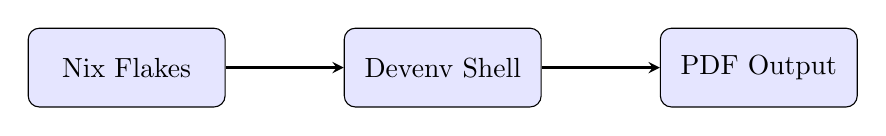
\begin{tikzpicture}[
			box/.style={draw, rectangle, rounded corners, minimum width=2.5cm, minimum height=1cm, align=center, fill=blue!10},
			arrow/.style={->, >=stealth, thick}
		]
		\node[box] (nix) {Nix Flakes};
		\node[box, right=1.5cm of nix] (devenv) {Devenv Shell};
		\node[box, right=1.5cm of devenv] (pdf) {PDF Output};

		\draw[arrow] (nix) -- (devenv);
		\draw[arrow] (devenv) -- (pdf);
	\end{tikzpicture}
	\caption{Hermetic LaTeX Compilation Pipeline}\label{fig:pipeline}
\end{figure}

\section{Code Listings}
Below is an example of a Nix expression used to configure the development shell:

\begin{lstlisting}[language=bash, caption={Build command with latexmk}]
# Compile main document to PDF
devenv shell build-pdf main.tex

# Or run live watch mode
devenv shell watch main.tex
\end{lstlisting}

\section{Conclusion}
Your LaTeX environment is ready to use! You can now edit \texttt{main.tex} and compile it instantly.

\bibliographystyle{plain}
\bibliography{references}

\end{document}
